\documentclass[12pt]{report}

\usepackage{commands}

\newcommand{\bld}[1]{{\mathbf{#1}}}

\begin{document}

\large

\begin{center}
 Math 585 Homework 1\\
 Due January 29\\
 By Marvyn Bailly\\
\end{center}

\normalsize

\hrule

%---------------%
%---Problem 1---%
%---------------%

%--Fix write up--$

\begin{problem}
    T1. Using an orthogonal polynomial basis, find the best least squares polynomial approximation of degree 2 to the function $f(t) = e^{-t}$ on the interval $[0, 1]$, i.e., find $p_2(t)$ that minimizes
    \[ 
        \int_0^1 \paren{f(t) - p_2(t)}^2dt.
    \]
    If the monomial basis is used, will the resulting polynomial be the same as the one obtained above? Explain.
\end{problem}

\begin{solution}
    
    \noindent
    We wish to find the best least squares polynomial approximation of degree 2 to the function $f(t) = e^{-t}$ on the interval $[0, 1]$, i.e., find $p_2(t)$ that minimizes
    \[ 
        \int_0^1 \paren{f(t) - p_2(t)}^2dt.
    \]
    For the orthogonal polynomial basis, let's use the Legendre polynomial basis which is given by
    \[ 
        \pi_0 = 1, \pi_1 = t, \pi_{j+1} = \frac{2j + 1}{j+1}t\pi_j(t) - \frac{j}{j+1}\pi_{j-1}(t) \implies \pi_2 = \frac{3}{2}t^2 - \frac{1}{2},
    \]
    which are in the interval $[0,1]$. Using the linear transformation $[0,1] \rightarrow [-1,1]$ by $2t - 1$, we get the basis to be
    \[ 
        \pi_0 = 1, \pi_1 = 2t-1, \pi_2 = \frac{3}{2}(2t - 1)^2 -\frac{1}{2}.
    \] 
    We know that the coefficients of the normal equations are given by
    \[ 
        c_j = \frac{(\pi_i,f)}{(\pi_i,\pi_i)},
    \]
    which yields
    \begin{align*}
        c_0 &= \frac{\int_0^1 e^{-t} dt}{\int_0^1 1^2 dt} = \frac{e-1}{e},\\
        c_1 &= \frac{\int_0^1 (2t - 1) e^{-t} dt}{\int_0^1 (2t - 1)^2 dt} = \frac{3 (e-3)}{e}, \\
        c_2 &= \frac{\int_0^1 \paren{\frac{3}{2}t^2 - \frac{1}{2}} e^{-t} dt}{\int_0^1 \paren{\frac{3}{2}t^2 - \frac{1}{2}}^2 dt} = 5 \left(7-\frac{19}{e}\right).
    \end{align*}
    Thus we have that
    \begin{align*}
        p_2(t) &= \sum_{i=0}^2c_i\pi_i\\ 
        &= \frac{3 (e-3) (2 t-1)}{e}+5 \left(7-\frac{19}{e}\right) \left(\frac{3}{2} (2 t-1)^2-\frac{1}{2}\right)+\frac{e-1}{e}\\
        &=  \frac{(210 e-570) t^2}{e}+\frac{(552-204 e) t}{e}+\frac{33 e-87}{e},        
    \end{align*} 

    which we can see makes a good approximation of $f(t)$
    \begin{center}
        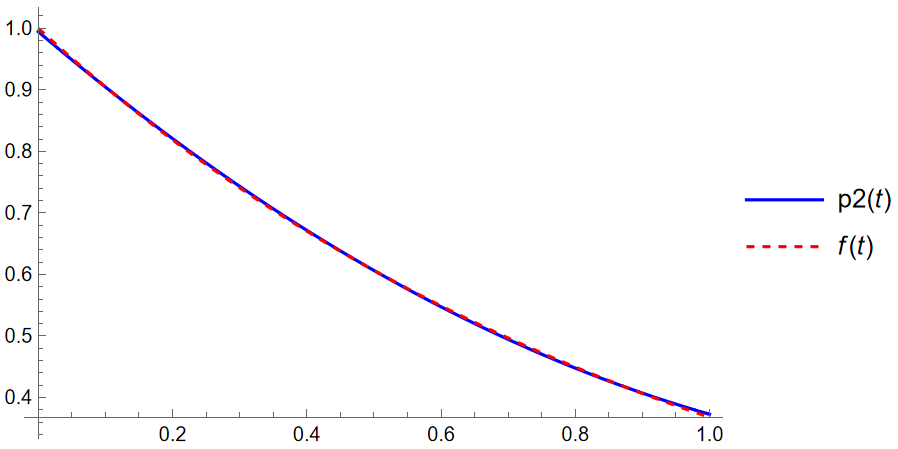
\includegraphics[width=.8\textwidth]{plots/Q1.PNG}
    \end{center}
    %monomial basis and polynomial basis generate the same basis. Look at page 65- FIX 
    We also note that the monomial basis projects into the same space as the polynomial basis and thus also satisfy the normal equations. We can also think about it as the monomial basis and polynomial basis both generate the same basis. Therefore there is no difference in the resulting polynomial as both options form the same basis. 


\end{solution}

%----------------------------------------------------------------------------------------------------%
%\vskip 20pt
\newpage

%---------------%
%---Problem 2---%
%---------------%

%--status--$

\begin{problem}
    T2. Given the four data points $(-1, 1), (0, 1), (1, 2)$ and $(2, 0)$, determine the interpolating cubic polynomial
    \begin{enumerate}
        \item[-] using the monomial basis;
        \item[-] using the Lagrange basis;
        \item[-] using the Newton basis.
    \end{enumerate}
    Show that the three representations give the same polynomial.
\end{problem}

\begin{solution}

    \noindent
    We wish to determine the interpolating cubic polynomial for the data points $(-1, 1), (0, 1), (1, 2)$ and $(2, 0)$.

    \begin{enumerate}
        \item [(a)] 
        First we wish to use a monomial basis. To do so, we need to solve for the coefficients of the Vandermonde matrix
        \[ 
            \begin{pmatrix}
                1 & -1 & 1 &-1\\
                1 & 0 & 0 & 0\\
                1 & 1 & 1 & 1\\
                1 & 2 & 4 & 8
            \end{pmatrix}\begin{pmatrix}
                c_0\\
                c_1\\
                c_2\\
                c_3
            \end{pmatrix} = \begin{pmatrix}
                1\\
                1\\
                2\\
                0
            \end{pmatrix}.
        \]
        Solving this system we get
        \[ 
            \bld{c} = \begin{pmatrix}
                1\\
                7/6\\
                1/2\\
                -2/3
            \end{pmatrix}.
        \]
        We know that the interpolating cubic polynomial takes the form of
        \[ 
            p_3(x) = \sum_{i=0}^{n}c_i f_i,
        \]
        Thus the interpolating cubic polynomial is given by
        \[ 
            p_3(x) = 1 + \frac{7}{6}x + \frac{1}{2}x^2 - \frac{2}{3}x^3.
        \]


        \item [(b)] Next we wish to use the Lagrange basis. We know that the Lagrange basis take the form
        \[ 
            l_i(x) = \prod_{j=0,j\neq i}^3 \frac{x - x_j}{x_i - x_j}, ~~ i = 0,1,2,3.
        \] 
        Thus we get the terms of the basis to be
        \begin{align*}
            l_0(x) &= -\frac{1}{6} x (x-1) (x-2),\\
            l_1(x) &= \frac{1}{2} (x+1)(x-1) (x-2),\\
            l_2(x) &= \frac{1}{2} (x+1)x(x-2), \\
            l_3(x) &= \frac{1}{6} (x+1)x(x-1).
        \end{align*}
        Then the interpolating cubic polynomial is given by
        \[ 
            p_3(x) = 1 \cdot -\frac{1}{6} x (x-1) (x-2) + 1 \cdot \frac{1}{2} (x+1)(x-1) (x-2) + 2 \cdot\frac{1}{2} (x+1)x(x-2).
        \]
        Note the this is the same as the monomial basis as
        \[ 
            -\frac{1}{6} (1-x) (2-x) x+(2-x) (x+1) x+\frac{1}{2} (1-x) (2-x) (x+1) = 1 + \frac{7}{6}x + \frac{1}{2}x^2 - \frac{2}{3}x^3.
        \]


        
        \item [(c)] Next we wish to use the Newton basis. To find the Newton basis, we can use the following table of divided difference        
        \begin{center}
            \begin{tabular}{lllll}
                $x$&  $f$&  &  &   \\
                \hline
                $-1$&  $1$&  &  &   \\
                $0$&  $1$&  $[-1,1]f$&  &   \\
                $1$&  $2$&  $[0,1]f$& $[-1,0,1]f$ &   \\
                $2$&  $0$&  $[1,2]f$&  $[-1,0,1]f$&  $[-1,0,1,2]f$
            \end{tabular}    
        \end{center}
        which yields
        \begin{center}
            \begin{tabular}{lllll}
                $x$&  $f$&  &  &   \\
                \hline
                $-1$&  $1$&  &  &   \\
                $0$&  $1$&  $0$&  &   \\
                $1$&  $2$&  $1$& $1/2$&   \\
                $2$&  $0$&  $-2$&  $-3/2$&  $-2/3$
            \end{tabular}    
        \end{center}
        Then the cubic interpolating polynomial is given by
        \[ 
            p_3(x) = \frac{1}{2} x (x+1)-\frac{2}{3} (x-1) x (x+1)+1 = -\frac{2 x^3}{3}+\frac{x^2}{2}+\frac{7 x}{6}+1,
        \]
        which is the same as the other two polynomials. We can also verify that this polynomial is this correct polynomial for the given data by plotting the points with the polynomial on Mathematica.
        \begin{center}
            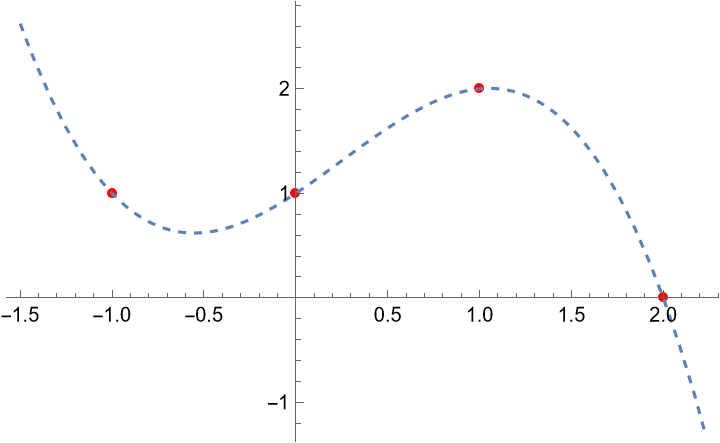
\includegraphics[width=.8\textwidth]{plots/Q2.png}
        \end{center}
    \end{enumerate}
\end{solution}

%----------------------------------------------------------------------------------------------------%
%\vskip 20pt
\newpage

%---------------%
%---Problem 3---%
%---------------%

%--status--$

\begin{problem}
    T3. Suppose $f$ is a function on $[0,3]$ for which one knows that
    \[ 
        f(0) = 1, f(1) = 2, f'(1) = -1, f(3) = f'(3) = 0.
    \]
    \begin{enumerate}
        \item [(a)] Estimate $f(2)$, using Hermite interpolation.    
        \item [(b)] Estimate the maximum possible error of the answer given in (a) if one knows, in addition, that $f \in C^5[0,3]$ and $|f^{(5)}(x)| \leq M$ on $[0,3]$. Express the answer in terms of $M$.
    \end{enumerate}

\end{problem}

\begin{solution}

    \noindent
    Consider the function $f$ on $[0,3]$ for which we know that
    \[ 
        f(0) = 1, f(1) = 2, f'(1) = -1, f(3) = f'(3) = 0.
    \]
    \begin{enumerate}
        \item [(a)]
        First we wish to estimate $f(2)$ using Hermite interpolation. We have the basis
        \[ 
            x_0, x_1,x_3,
        \]
        which we must extend to 
        \[ 
            x_0, x_1, x_1, x_3, x_3,
        \]
        for Hermite interpolation. Using the extended basis, we can construct the following table of divided difference
        \begin{center}
            \begin{tabular}{llllll}
                $x$&  $f$&  &  &   \\
                \hline
                $0$&  $1$&  &  &   \\
                $1$&  $2$&  $[x_0,x_1]f$&  &   \\
                $1$&  $2$&  $[x_1,x_1]f = f'(1)$& $[x_0,x_1,x_1]f$ &   \\
                $3$&  $0$&  $[x_3,x_1]f$&  $[x_1,x_1,x_3]f$&  $[x_0,x_1,x_1,x_3]f$\\
                $3$&  $0$&  $[x_1, x_3, x_3]f = f'(3)$& $[x_1,x_3,x_3]f$& $[x_1,x_1,x_3,x_3]f$&$[x_0,x_1,x_1,x_3,x_3]f$
            \end{tabular}    
        \end{center}
        which yields
        \begin{center}
            \begin{tabular}{llllll}
                $x$&  $f$&  &  &   \\
                \hline
                $0$&  $1$&  &  &   \\
                $1$&  $2$&  $1$&  &   \\
                $1$&  $2$&  $-1$& $-2$ &   \\
                $3$&  $0$&  $-1$&  $0$&  $2/3$\\
                $3$&  $0$&  $0$& $1/2$& $1/4$&$-5/36$
            \end{tabular}    
        \end{center}
        We know that the Hermite interpolation polynomial is of the form
        \[ 
            p_4(x) = \sum_{i=0}^4 [x_0,\dots,x_i]f \prod_{j=0}^{i-1}(x - x_j).
        \]
        Plugging in our values from the table gives
        \[ 
            p_4(x) = 1 + x - 2(x)(x-1) + \frac{11}{12}x(x-1)^2 + \frac{5}{36}(x)(x-1)^2(x-3).
        \]
        We can verify this polynomial hits all the points with the following graph generated in Mathematica.
        \begin{center}
            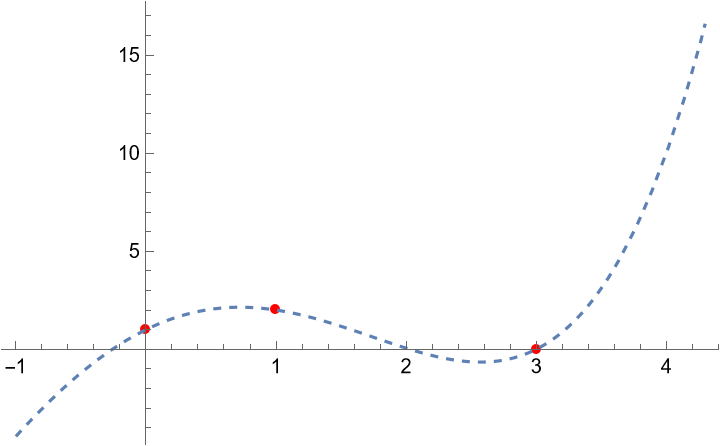
\includegraphics[width=.8\textwidth]{plots/Q3.png}
        \end{center}
        Therefore we can approximate $f(2)$ to be
        \[ 
            f(2) \approx p_4(2) = \frac{11}{18}.
        \]

        \item [(b)]
        Next we wish to estimate the maximum possible error of the answer in (a) using the additional information that $f \in C^5[0,3]$ and $|f^{(5)}(x)| \leq M$ on $[0,3]$. Note that the general error term for our Hermite interpolation polynomial is 
        \[ 
            f(x) - p_4(x)  = \frac{f^{(5)}(x)}{5!}(x)(x-1)^2(x-3)^2.
        \]
        Thus to get the maximum possible error observe that
        \[ 
            |f(2) - p_4(2)| = \abs{\frac{f^{(5)}(2)}{5!}(2)(2-1)^2(2-3)^2} = \abs{\frac{f^{(5)}(2)}{60}} \leq \frac{M}{60}.
        \]
        Therefore the maximum possible error is
        \[ 
            \frac{M}{60}.
        \]
        
    \end{enumerate}
\end{solution}

%----------------------------------------------------------------------------------------------------%
%\vskip 20pt
\newpage

%---------------%
%---Problem 4---%
%---------------%

%--status--$

\begin{problem}
    T4. Let the subdivision $\Delta$ of $[a; b]$ be given by
    \[
        \Delta : a = x_1 < x_2 < \cdots < x_{n-1} < x_n = b, n \geq 2,
    \]
    and let $f_i = f(x_i), i = 1,2,\dots,n$ for some function $f$. Suppose you want to interpolate this data by a quintic spline $s_5(f;\cdot)$ (a piecewise fifth degree polynomial of smoothness class $C^4[a,b]$). By counting the number of parameters at your disposal and the number of conditions imposed, state how many additional conditions (if any) you expect are needed to make $s_5(f;\cdot)$ unique.
\end{problem}

\begin{solution}

    \noindent
    Let the subdivision $\Delta$ of $[a; b]$ be given by
    \[
        \Delta : a = x_1 < x_2 < \cdots < x_{n-1} < x_n = b, n \geq 2,
    \]
    and let $f_i = f(x_i), i = 1,2,\dots,n$ for some function $f$. If we want to interpolate this data by a quintic spline $s_5(f;\cdot)$, we need six coefficients for the $n-1$ intervals. Thus there are $6(n-1)$ degrees of freedom. For each of the $n-1$ intervals, we have two conditions to match the endpoints. For each of the $n-2$ interior points, we require that the derivative up to the fourth match, thus there are four conditions. Thus we have $2(n-1) + 4(n-2) = 6n - 10$ conditions. Since we need the number of conditions to match the degree of freedom to have a unique solution, we need $4$ additional conditions. 
\end{solution}

%----------------------------------------------------------------------------------------------------%
%\vskip 20pt
\newpage

%---------------%
%---Problem 5---%
%---------------%

%--status--$

\begin{problem}
    C1. Consider the Runge function
    \[ 
        f(x) = \frac{1}{1 + x^2}, ~~ x\in[-5,5].
    \]
    \begin{enumerate}
        \item [-]
        Plot the Lagrange interpolating polynomials using equidistant nodes $x_i = -5 + \frac{10i}{n}$, $i= 0, \dots,n$. Try $n=5,10,15,$ and $20$. 
        
        \item [-]
        Plot the Lagrange interpolating polynomials using Chebyshev nodes $x_i = 5\cos\paren{\frac{(2i + 1)\pi}{2(n+1)}}$, $i= 0, \dots,n$. Try $n=5,10,15,$ and $20$.
        
        \item [-]
        Plot the cubic complete splines using equidistant nodes $x_i = -5 + \frac{10i}{n}$, $i= 0, \dots,n$. Try $n=5$ and $10$. You may use MATLAB's spline.
        
    \end{enumerate}
    Generate one plot for each of the three cases, respectively. For each case, plot also $f$ as a reference.
\end{problem}

\begin{solution}

    \noindent
    Consider the Runge function 
    \[ 
        f(x) = \frac{1}{1 + x^2}, ~~ x\in[-5,5].
    \]
    I used the following MATLAB code to generate Figure 1 which plots the Lagrange interpolating polynomials using equidistant nodes $x_i = -5 + \frac{10i}{n}$, $i= 0, \dots,n$ for $n=5,10,15,$ and $20$. Figure 2 which plots the Lagrange interpolating polynomials using Chebyshev nodes $x_i = 5\cos\paren{\frac{(2i + 1)\pi}{2(n+1)}}$, $i= 0, \dots,n$ for $n=5,10,15,$ and $20$. And Figure 3 which plots the cubic complete splines using equidistant nodes $x_i = -5 + \frac{10i}{n}$, $i= 0, \dots,n$ for $n=5$ and $10$ using MATLAB's spline.

    \begin{figure}
        \center
        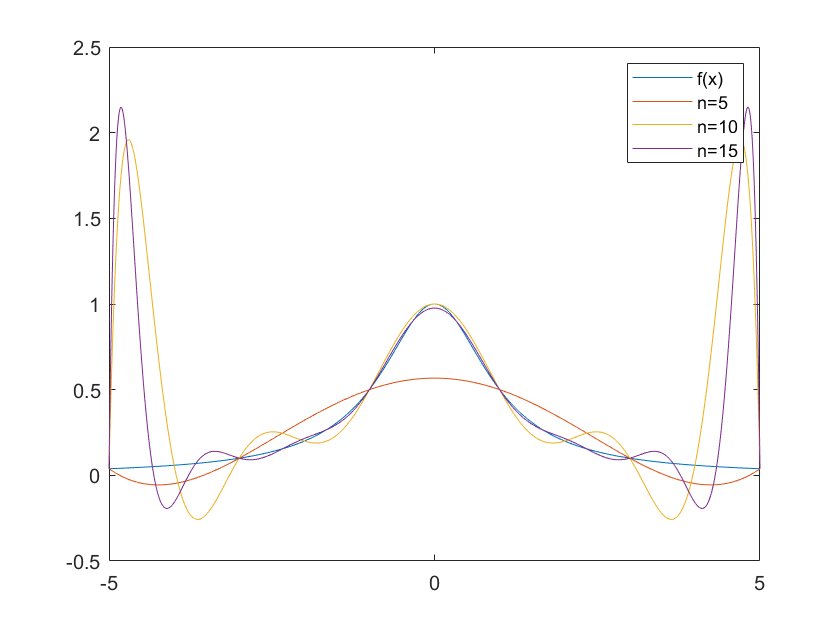
\includegraphics[width = 0.49\linewidth]{plots/Q5a1.png}
        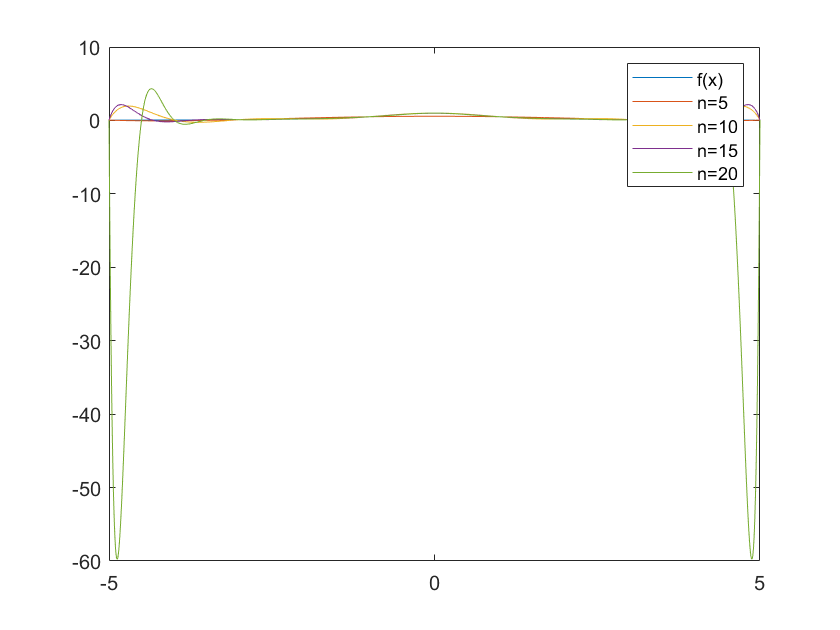
\includegraphics[width = 0.49\linewidth]{plots/Q5a2.png}
        \caption{Lagrange interpolating polynomials using equidistant nodes.}
    \end{figure}


    \begin{figure}
        \center
        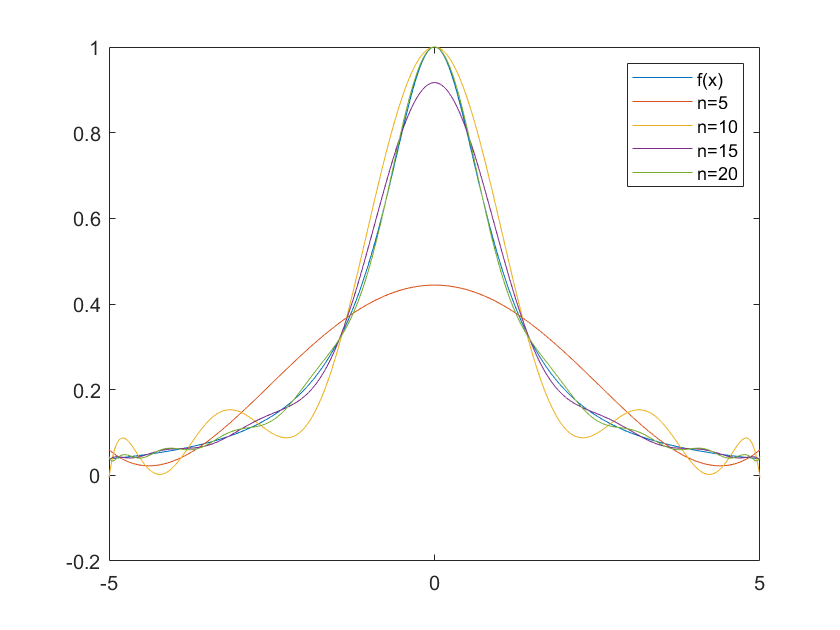
\includegraphics[width = 0.6\linewidth]{plots/Q5b.png}
        \caption{Lagrange interpolating polynomials using Chebyshev nodes.}

        \center
        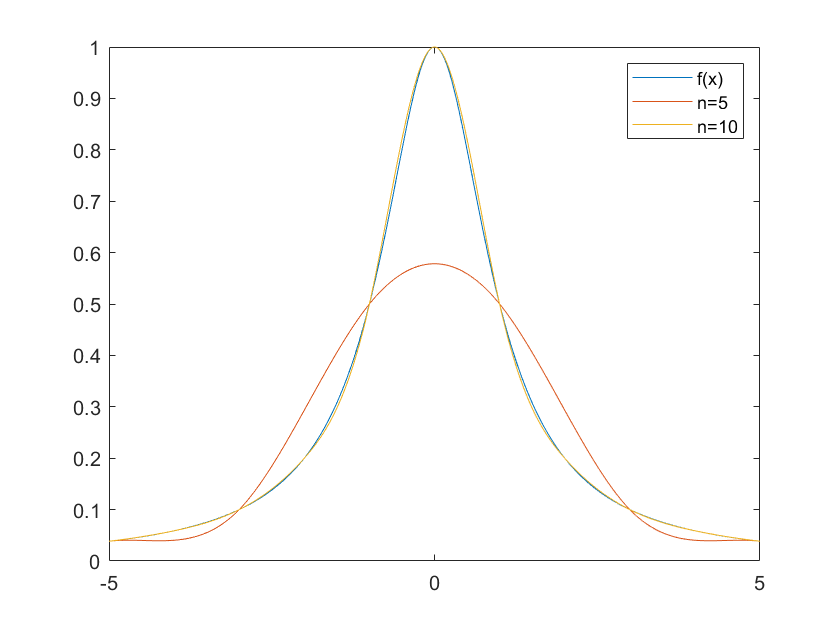
\includegraphics[width = 0.6\linewidth]{plots/Q5c.png}
        \caption{Cubic complete spines using equidistant nodes.}
    \end{figure}

    \newpage
    \noindent
    {\bf Lagrange Function:}
    \begin{verbatim}
    function y = getLagrange(xvals,yvals,x)
        n = length(xvals);
        m = length(x);
        basis = ones(m,n);
        y = zeros(m,1);
        
        for i=1:n
            for j=1:n
                if i~=j
                    basis(:,i) = basis(:,i).*(x-xvals(j))./(xvals(i) - xvals(j));
                end
            end 
        end
        
        for i=1:n
            y = y+yvals(i)*basis(:,i);
        end
    end
    \end{verbatim}

    \noindent
    {\bf Main Code:}
    \begin{verbatim}
        nvals = [5,10,15,20];
        x = linspace(-5,5,1000)';
        y = 1./(1 + x.^2);

        figure(1)
        plot(x,y)
        hold on

        %Part (a)
        for i=1:3
            n= nvals(i);
            xvals = -5 + (10/n)*(0:n);
            yvals = 1./(1 + xvals.^2);
            plot(x, getLagrange(xvals,yvals,x))
        end
        legend("f(x)","n=5","n=10","n=15","n=20");
        hold off

        %Part (b)
        figure(2)
        plot(x,y) 
        hold on

        for i=1:4
            n= nvals(i);
            xCheb = 5*cos(pi*(2*(0:n) +1)/(2*(n+1)));
            yCheb = 1./(1 + xCheb.^2);
            plot(x, getLagrange(xCheb,yCheb,x))
        end
        legend("f(x)","n=5","n=10","n=15","n=20");
        hold off

        %Part (c)
        figure(3)
        plot(x,y) 
        hold on

        for i=1:2
            n= nvals(i);
            
            xSpline = -5 + (10/n)*(0:n);
            ySpline = 1./(1 + xSpline.^2);
            
            plot(x,spline(xSpline,[5/338 ySpline -5/338],x));
        end
        legend("f(x)","n=5","n=10");
        hold off
    \end{verbatim}

\end{solution}

%----------------------------------------------------------------------------------------------------%
%\vskip 20pt
\newpage

\end{document}